\subsection{Relevant Technologies}
% compare the available technologies and propose how to apply them to our system

\subsubsection{Sensor Ranging}
% Toby - sensors, haptics basic goal
\noindent Ranging sensors are used to provide distance-to-obstacle information for a plethora of products today. They are popularly found in robotics, where they are able to provide awareness of the surroundings, vehicles, where they enable autonomous navigation, or for smart facility and home solutions, where they detect movement and are used to trigger various actions. FORWARD requires sensors to enable safe navigation and it is thus appropriate to examine the technologies available to determine which to install on the walker. The intent also is two-fold in that it is desired to gain knowledge of what is attainable, namely what information about the surroundings can we provide our processor and how accurate and insightful can that information be. Note that, FORWARD does not implement features of user health status or tracking and so we do not examine GPS as a relevant technology. FORWARD navigates autonomously, and it will do this by use of \textbf{\textit{time-of-flight sensing}}.\\

\noindent \underline{\textit{Ultrasonic}} There are differing variations of ultrasonic sensing technology, mainly varying by their 1) transmitting and receiving hardware, which can be realized as mono or multistatic, 2) emission and detection capability, which stipulates their active or passive status, and 3) their operating frequency \cite{sonar-type}. As far as whether the hardware comes in the form of a multistatic setup or a single transceiver (emits and receives ultrasound), FORWARD's requirements do not necessarily rule out one or the other. Monostatic could be slightly more conducive to mounting on the walker legs and help retain a lower profile because of their smaller (2x) dimensions.\\

\begin{figure}[H]
	\centering
	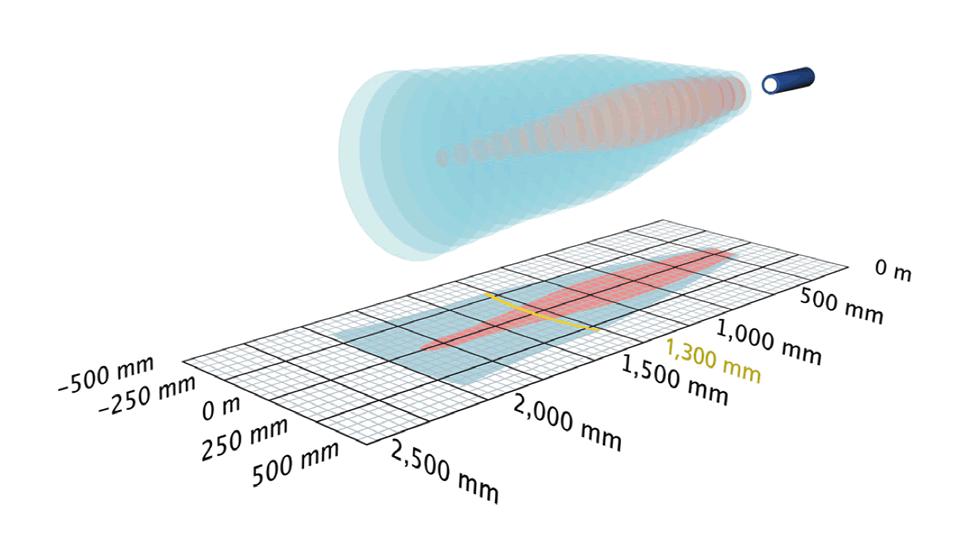
\includegraphics[width=0.7\textwidth]{./Images/cool-ultrasonic-directivity.png}
	\caption{\label{fig:cool-directivity}Ultrasonic Directivity \cite{coolUltraDirect}}
\end{figure}

\noindent \underline{\textit{LiDAR}} We deploy LiDAR in the context of this project as 1) oriented laterally, 2) topographic, and 3) using the scanning method fixed/solid-state (as opposed to swivel or rotating) without flash \cite{lidar-type} (because we are not desiring to create maps). As designers, we must also consider that LiDAR reliability may be affected by the reflectivity of the target objects and ambient lighting of the surroundings. This is one of the primary reasons both sound and light sensing applications are under consideration. Note, figure \ref{fig:lidarazimuth} shows a scanning LiDAR. In this project, the azimuth and elevation difference are both negligible, as the light beam is single-point. Scanning would require another subsystem with servomotors, which is not in specification or budget. By utilizing both sonic and laser sensors however, we can cover a wider range of azimuth. As discussed earlier, the camera is able to cover more elevation for detection.\\

\begin{figure}[H]
	\centering
	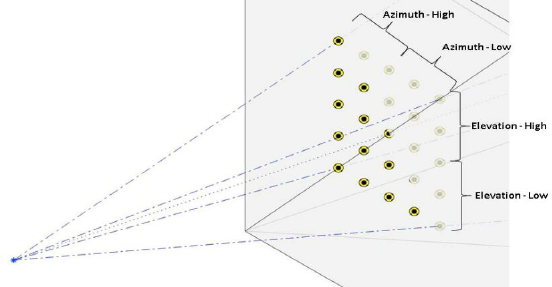
\includegraphics[width=0.7\textwidth]{./Images/FOV-scanning-LIDAR.png}
	\caption{\label{fig:lidarazimuth}Scanning LiDAR FOV \cite{coolLiDARfov}}
\end{figure}

% advanced goal
\subsubsection{Walker Stability} \label{sssec:3_2stability}
\noindent \underline{\textit{Inertial Measurement}} Units are comprised of a magnetometer and accelerometer, which obtain the acceleration and body rate readings of the walker. This is traditionally done by a reading a gyroscope rotation or looking at the magnetic field. It could be greatly beneficial to gain this data, not only for analytical use, but for functionality. Some of the stretch requirements include curb lifting, fall prevention, and incline decline adaptation. With an IMU on-board, the walker can respond appropriately to each scenario. For instance, when lifting over a curve, there can be a certain pitch angle limit imposed to prevent tipover. This is expanded in a similar fashion for fall prevention, where if the user leans too much on the handlebars and causes a tipover, the IMU data can inform the motors of a decision. Finally, the IMU angles are also useful when traversing over inclines or declines. The body rates may also be useful for stability while turning, smoothing the yaw maneuver.\\

\noindent \underline{\textit{Sonar vs. LiDAR for Detection}} As gleaned from \cite{sonar-vs-lidar}, ultrasonic sensors are advantageous for their low cost, simple digital input and output, and wider FOV. However, they lack in their exposure to environment, slower response time, and larger physical size. LiDAR sensors on the other hand, are small and lightweight, and have a fast response time. However, they generally cost more and have a more narrow FOV because of their environmental seal and laser physics.\\

\noindent \underline{\textit{Balanced Sensor Informants}} When comparing the selling points of cameras and traditional sensing methods, we see that each have their advantages. Cameras allow for the most detailed information about the shape and size of the obstacle, but they rely on a lens that can become dirty. The camera may also not operate well in lowlight environments. By still including the ultrasonic and LiDAR, FORWARD can always sense obstacles and have multiple informants. Each sensing method covers the next. When ultrasonic may be affected by wind, the LiDAR is not. When the reflectivity of an object may obscure the LiDAR, the sound waves can still detect. \cite{camera-vs-sensor}.\\

\noindent \underline{\textit{Sensor Fusion}} Implementation of sensor fusion to converge on a most accurate range solution would not be beneficial derived from the ultrasonic and LiDAR outputs, because they should both give nearly identical readings, and thus, leaving no need for fusion. However, it could greatly enhance the computer vision by allowing it to not only identify and classify hazards, but also aid with range detection. The range given by the camera's depth perception could be fused with the more reliable range readings from the front of the walker to further confirm the presence and distance of obstacles. Additionally, the camera could inform the avoidance subsystem of ultrasonic and LiDAR range data to for any reason, ignore.\\

% Matthew - MCU, computer vision, audio
\subsubsection{Computer Vision Object Detection}
\noindent The Object Detection section of our system will be used to identify and alert the user of their surrounding environment. Because of this, we will need our system to be real-time and highly accurate. The main model used for this is known as YOLO. Many of the current object detection applications implement a YOLO model to process the image data. \\

\noindent The algorithm works based on the following four approaches: Residual blocks, Bounding box regression, Intersection Over Unions or IOU for short, Non-Maximum Suppression. Residual blocks divide the image into an N by N grid, in which each section becomes a sub-problem. The algorithm then seeks to calculate a resulting vector through bounding box regression. The vector contains the confidence of an objects presence (pc), the image center (bx, by), and the area of the object (bh, bw), resulting in Y = [pc, bx, by, bh, bw, c1, c2]. c1 and c2 are the possible classifications. It's also worth nothing the bh and bw can be greater then the size of the grid. The algorithm then uses intersection over unions and non-maximum suppression to determine what information has the greatest meaning, and thus, we have a prediction. \\

\noindent It should also be said that the above describes how to model runs in real time applications, and operates on the assumption that the model has been trained, which in many cases, it has been trained on the MSCOCO data set. \\

\subsubsection{Current Audio Feedback Technologies}
\noindent The Audio Feedback portion of our project needs careful consideration given it's importance in providing the user with audio cues for their environment all the while still being implemented on an embedded MCU, which is likely to contain limited resources. The MCU's considered for this project all contain Bluetooth capabilities and so we will be diving into research for successful products for our application. \\

\noindent \underline{\textit{Bluetooth}} \cite{bluetooth} is another key component to the success of our project. To successfully communicate important visual information to our user, we need to do so audibly; and to communicate audibly without interfering with the user with wires. Due to the target users being visually impaired, it is crucial to limit any possible hazards - thus creating a large need for Bluetooth technology. Bluetooth is a wireless communication protocol that transmits on a range centered at 2.45 GHz. Bluetooth is designed to connect clients of short distance, usually 0 to 30 feet, and can be on up to 79 channels. Bluetooth \cite{bluetoothHow} is also a very low power technology, which makes it close range and secure, with negligible interference among different users. Bluetooth protocol allows for it to be very efficient through the concept of \textit{spread-spectrum frequency hopping}. This concept is picture below in figure 8. Spread-spectrum frequency hopping is when two devices want to communicate, they look for a channel that is available by hopping frequencies. This concept also adds to the security and non-interfering capabilities of Bluetooth because many Bluetooth devices will do this up to thousands of times per second. Bluetooth is mainly used to connect electronics of close ranges, and is commonly used for audio applications - which will be our use as well. \\

\begin{figure}[H]
	\centering
	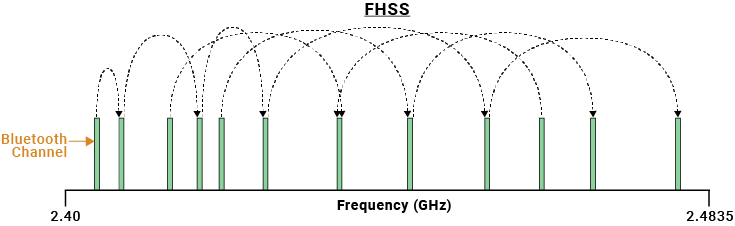
\includegraphics[width=1\textwidth]{./Images/bluetooth-freq-hop.png}
	\caption{\label{fig:bluetooth-freq-hop}Bluetooth Spread-spectrum Frequency Hopping}
\end{figure}

\noindent The following technologies were considered and researched as a solution to our audio feedback system: \\

\noindent The first technology considered is based upon \underline{\textit{Bone Conduction technology}} \cite{BoneConductionRef}. Bone conduction technology allows users to perceive sound through the vibrations of the bones in the inner ear. One of the main benefits is that audio information can be received even if the ears canals are blocked, which allows for definite communication to the user. Conversely, It also address one of our biggest goals with this system by not obstructing the users ears ways. The bone conduction technology ear pieces sit on the outside of the ear, providing complete freedom for the users ear. Some secondary benefits of bone conduction is increased clarity and reduced background noise as well. While this technology is very advantageous for our goals, some health and comfort disadvantages exist. Prolonged and extraneous use of this technology has been seen to cause hearing loss, vertigo, and tinnitus. This technology can also become uncomfortable to wear for extended periods of time. On average, these headphones have 8 to 12 hours of play time and bluetooth capabilities.  \\

\noindent The second technology considered is \underline{\textit{Ambient Sound Earbuds}}. In order to use a headphone that blocks the ear canal - it would require the use of ambient sound technology to still allow the sound from the outside world. The reason this is of importance is to allow the user to still maintain audible awareness of their immediate surroundings, which if hindered to much, can be severely hazardous. Albeit, even the current state of ambient sound technologies is not the greatest, and can introduce risk for the user having one or two of these earbuds in. The technical  specifications for these product include - 5 to 8 hours of playtime. They cost \$25 to \$50 which can be in our expected range and affordable. \\

\noindent The third technology considered is \underline{\textit{Open Air Bluetooth Speakers}}, coming directly from the chassis on the system. In general, bluetooth speakers are a highly developed technology, which means they are highly reliable with a wide variety of options for our needs. They can cost anywhere from \$20 to \$300, and can run 8 to 20 hours of battery life. The main downside though has public disturbance implications as it would impede on everyone's daily life around the user. The other downside is we introduce risk by not directly relaying the information to the user, such as in a loud room. \\

% Morgan - Power supply, motors, motor shield, steering, braking
\subsubsection{Motor Shield/Driver}
